\documentclass[]{elsarticle} %review=doublespace preprint=single 5p=2 column
%%% Begin My package additions %%%%%%%%%%%%%%%%%%%
\usepackage[hyphens]{url}

  \journal{Journal of Applied Ecology} % Sets Journal name


\usepackage{lineno} % add
  \linenumbers % turns line numbering on
\providecommand{\tightlist}{%
  \setlength{\itemsep}{0pt}\setlength{\parskip}{0pt}}

\usepackage{graphicx}
\usepackage{booktabs} % book-quality tables
%%%%%%%%%%%%%%%% end my additions to header

\usepackage[T1]{fontenc}
\usepackage{lmodern}
\usepackage{amssymb,amsmath}
\usepackage{ifxetex,ifluatex}
\usepackage{fixltx2e} % provides \textsubscript
% use upquote if available, for straight quotes in verbatim environments
\IfFileExists{upquote.sty}{\usepackage{upquote}}{}
\ifnum 0\ifxetex 1\fi\ifluatex 1\fi=0 % if pdftex
  \usepackage[utf8]{inputenc}
\else % if luatex or xelatex
  \usepackage{fontspec}
  \ifxetex
    \usepackage{xltxtra,xunicode}
  \fi
  \defaultfontfeatures{Mapping=tex-text,Scale=MatchLowercase}
  \newcommand{\euro}{€}
\fi
% use microtype if available
\IfFileExists{microtype.sty}{\usepackage{microtype}}{}
\usepackage[margin=1.4in]{geometry}
\bibliographystyle{elsarticle-harv}
\usepackage{longtable}
\ifxetex
  \usepackage[setpagesize=false, % page size defined by xetex
              unicode=false, % unicode breaks when used with xetex
              xetex]{hyperref}
\else
  \usepackage[unicode=true]{hyperref}
\fi
\hypersetup{breaklinks=true,
            bookmarks=true,
            pdfauthor={},
            pdftitle={Invasive mesopredator release},
            colorlinks=false,
            urlcolor=blue,
            linkcolor=magenta,
            pdfborder={0 0 0}}
\urlstyle{same}  % don't use monospace font for urls

\setcounter{secnumdepth}{5}
% Pandoc toggle for numbering sections (defaults to be off)

% Pandoc citation processing

% Pandoc header
\usepackage{setspace}\doublespacing



\begin{document}
\begin{frontmatter}

  \title{Invasive mesopredator release}
    \author[UOM]{Matthew W. Rees\corref{1}}
   \ead{matt.wayne.rees@gmail.com} 
    \author[CEC]{Jack H. Pascoe}
  
    \author[UOM]{Brendan A. Wintle}
  
    \author[ARI]{Alan Robley}
  
    \author[CEC]{Mark Le Pla}
  
    \author[CEC]{Emma K. Birnbaum}
  
    \author[UOM]{Bronwyn A. Hradsky}
  
      \address[UOM]{Quantitative \& Applied Ecology Group, School of Ecosystem and Forest Science, The University of Melbourne, Parkville, VIC, Australia}
    \address[CEC]{Conservation Ecology Centre, Otway Lighthouse Rd, Cape Otway, VIC, Australia}
    \address[ARI]{Department of Environment, Land, Water and Planning, Arthur Rylah Institute for Environmental Research, Heidelberg, Australia}
      \cortext[1]{Corresponding Author}
  
  \begin{abstract}
  \begin{enumerate}
  \def\labelenumi{\arabic{enumi}.}
  \item
    Background.
  \item
    Methods.
  \item
    Results.
  \item
    \emph{Synthesis and applications.}
  \end{enumerate}
  \end{abstract}
   \begin{keyword} Camera trap; Felis catus; invasive predator; interspecific competition; mesopredator release; population density; spatial capture-recapture; spatial mark-resight; species interactions; Vulpes vulpes.\end{keyword}
 \end{frontmatter}

\parskip=12pt

\newpage

\hypertarget{introduction}{%
\section{INTRODUCTION}\label{introduction}}

Understanding species interactions is critical for effective invasive species management (Zavaleta et al., 2001).
When several invasive species co-occur, management actions that suppress the dominant invasive species may inadvertently benefit subordinate invasive species (Jackson, 2015; Kuebbing \& Nuñez, 2015).
Subordinate invasive species may be released from direct top-down pressure following a decline in the dominant predator or benefit indirectly from an increase in availability of shared resources (often referred to as mesopredator or competitor release - Crooks \& Soulé, 1999; Doherty \& Ritchie, 2017; Ruscoe et al., 2011).
The release of a subordinate invasive species, particularly predators, can have serious negative implications for native taxa and ecosystem function (Ballari et al., 2016; Courchamp et al., 1999).
However, integrated predator management is often far more costly and less feasible than single species control, and so it is important to identify the extra cost if justified (Bode et al., 2015).

Most knowledge of predator interactions stems from unreplicated ``natural experiments'' (e.g.~range contractions - Crooks \& Soulé, 1999) or ad-hoc management interventions (e.g.~invasive species eradications - Rayner et al., 2007).
However, the occurrence, nature (positive or negative, direct or indirect) and strength of species interactions can vary among species assemblages, predation risk, environmental productivity, management regimes, and other landscape contexts (Alston et al., 2019; Finke \& Denno, 2004; Hastings, 2001).
Replicating management programs in an experimental framework is logistically challenging, but important for understanding these complexities, discriminating between plausible hypotheses and producing generalisable results in order to inform effective pest management (Christie et al., 2019; Glen \& Dickman, 2005; Smith et al., 2020).

Unbiased estimates of invasive predator density are vital for inferring native prey impacts on and for setting meaningful control targets (Moseby et al., 2019). However, controversy around the mesopredator release hypothesis has stemmed from the inability of traditional survey approaches to separate behavioural and numerical population processes (Hayward et al., 2015; Stephens et al., 2015).
These nonspatial approaches arbitrarily divide continuous landscapes into discrete spatial sampling units, but highly mobile predators can easily break model assumptions by crossing these (Efford \& Dawson, 2012).
Additionally, the suppression of an apex predator may change the behaviour and density of a mesopredator, both of which impact detection rates (Broadley et al., 2019; Rogan et al., 2019).
And so, even with experimental designs, it is difficult to interpret changes in unidentified counts or presence-absence records of mesopredators in relation to apex predators.
While spatially explicit capture-recapture methods have been developed to robustly estimate predator density by separating out behavioural and observational processes from population density, they have seldom been used experimentally or to investigate multispecies interactions (although, see Forsyth et al., 2019).

Predation by two invasive species, the red fox \emph{Vulpes vulpes} and feral cat \emph{Felis catus}, has played a major role in Australia's high rates of mammalian extinction (Woinarski et al.~2019).
Integrated invasive predator management programs are rare.
Introduced red foxes (hereafter foxes) are far more commonly controlled than feral cats, as they are more susceptible to poison-baiting, have greater direct economic impacts and fewer legal impediments to their control (McLeod \& Saunders, 2014; Reddiex et al., 2007).
Nonetheless, feral cats are one of the most widespread and damaging vertebrate species (Doherty \& Ritchie, 2017; Legge et al., 2020; Medina et al., 2011).
As foxes are larger-bodied (\textasciitilde2 kg difference) and have high dietary overlap with feral cats (Catling, 1988; Glen et al., 2011; Short et al., 1999), the mesopredator release hypothesis predicts that feral cat impacts will increase as fox populations are managed (Soulé et al., 1988).
This is alarming because feral cats are extremely difficult to manage in open populations (Fisher et al., 2015; Lazenby et al., 2015).

Evidence that foxes suppress feral cats is inconclusive (Hunter et al., 2018).
In parts of Australia where the native apex mammalian predator (the dingo \emph{Canis familiaris}) is functionally extinct and introduced red foxes are the largest terrestrial mammalian predator, four studies have observed an increase in feral cat detections following fox control (Marlow et al., 2015; Risbey et al., 2000; Stobo-Wilson et al., 2020).
However, two other studies in similar systems did not see any change (Molsher et al., 2017; Towerton et al., 2011).
One study with spatial replication detected an increase at one site but not another (Davey et al., 2006), and one study observed a decrease in feral cat activity (Claridge et al., 2010).
No previous study has directly estimated feral cat density in response to fox control.

In this study, we experimentally investigated the role of introduced foxes in top-down suppression of feral cat density in two regions of south-eastern Australia.
Foxes and feral cats are the only functional terrestrial mammalian predators in these regions, and each region included at least one area in which foxes were subject to continuous lethal poison-baiting (hereafter ``impact landscape''), and a paired area were foxes were not controlled (hereafter ``non-impact landscape'').
This allowed a sharp focus on the interactions between the two invasive predators, across a gradient of apex predator (fox) occupancy and landscape productivity.
We tested for a direct effect of fox control on feral cat density using traditional experimental approaches: a replicated Control-Impact design in the region with long-term fox control, and a Before-After Control-Impact Paired Series (BACIPS) design in the region with newly implemented fox control.
We also tested for direct associations between feral cat density and spatial fox occupancy (derived using generalised additive models) in each region, as well as investigated the relative importance of fine or broad scale fox measurements.
In accordance with the mesopredator release hypothesis, we predicted that (1) fox control would increase feral cat density, and (2) feral cat density would be negatively correlated with spatial fox occupancy.
We based inference on spatial mark-resight models of feral cat density and information criteria methods.

\newpage

\hypertarget{materials-and-methods}{%
\section{MATERIALS AND METHODS}\label{materials-and-methods}}

\hypertarget{study-area}{%
\subsection{Study area}\label{study-area}}

We conducted our study across two regions of south-west Victoria, Australia (Fig. \ref{fig:map}). The native temperate forests in both regions are fragmented to varying degrees, primarily by livestock farming and tree plantations. Although once widespread, dingoes are now absent throughout, and a native mesopredator, the tiger quoll \emph{Dasyurus maculatus}, is long absent from the Glenelg region and recently absent in the Otway Ranges (last sighted in 2014 despite extensive camera-trapping). The terrestrial mammalian predator guild is therefore depauperate, with the introduced fox and feral cat being the primary functional mammalian terrestrial predators; birds of prey and snakes are the only other predators present.

Our study landscapes in the Glenelg region, Gunditjmara country, are primarily lowland forest (with an overstorey of \emph{Eucalyptus obliqua} and \emph{E. ovata}, a sparse midstorey and a fern-rich understorey) and heathy woodland (with an overstorey of \emph{E. baxteri s.l.} and \emph{E. willisii}, a sparse midstorey and a diverse understorey of narrow or ericoid-leaved shrubs). It has gently undulating terrain and frequently experiences prescribed burns and wildfires, creating a mosaic of fire histories and vegetation complexity. The area receives an average annual rainfall of 700 mm, with average minimum temperatures of 8.1°C and maximum of 17.6°C (\emph{Bureau of Meteorology}, 2021).

Our study landscapes in the Otway region were in the western section of the Otway Ranges, Gadubanud country. Here, the vegetation is a mosaic of shrubby wet forest and cool temperate rainforest, with an overstorey of tall eucalyptus species (primarily \emph{E. regnans}), \emph{Acacia melanoxylon} and \emph{Nothofagus cunninghamii}. The midstorey is dominated by tree ferns, \emph{Acacia verticillata}, \emph{Pomaderris aspera} and \emph{Olearia argophylla}. The understorey predominantly comprises a dense layer of ferns and graminoids but can be relatively sparse in steep rainforest gullies. Maximum daily temperatures average 19.3°C in summer and 9.5°C in winter; annual rainfall averages 1955 mm (\emph{Bureau of Meteorology}, 2021). This region rarely experiences fire and is nearly ten times more rugged (based on the terrain ruggedness index (Riley et al., 1999) averaged within a 10 m radius of each camera-trap site).

\hypertarget{lethal-fox-control}{%
\subsection{Lethal fox control}\label{lethal-fox-control}}

Across broad sections of each region, government land managers conduct ongoing fox control for biodiversity conservation. Manufactured poison baits (FoxOff, Animal Control Technologies, Somerton) containing 3 mg of sodium mono-fluroacetate (1080) are buried at a depth of 10 cm at 1-km intervals along accessible forest tracks and roads (Fig. \ref{fig:map}). Different road densities across the two regions therefore result in variable poison-bait densities. In the Glenelg region, fox control in the impact landscapes has been ongoing since October 2005, with baits checked and replaced fortnightly (Robley et al., 2014). In the Otway region, baiting commenced in the impact landscape in November 2017. Poison baits were replaced weekly for six weeks until December 2017, before changing to monthly bait replacement until July 2018. The fox control program then lapsed for approximately six months until December 2018 due to logistical constraints, when monthly bait replacement recommenced for the duration of our study (Fig. S1).

\hypertarget{study-design-and-camera-trapping}{%
\subsection{Study design and camera-trapping}\label{study-design-and-camera-trapping}}

We designed experiments around the implementation of fox poison-baiting in each region. We simultaneously surveyed one impact and one non-impact landscape at a time using camera-traps. Each landscape pair was chosen based on similarity in landscape context, namely vegetation groups, with the aim of maintaining spatial independence with respect to predator range movements.

In the Glenelg region, we used a replicated control-impact design to test for differences in areas that have been poison-baited for foxes for more than 13 years compared with unbaited areas. We deployed a pair of camera-trapping grids in Cobboboonee National Park (impact) and Annya State Forest (non-impact) in January -- April 2018, then moved these cameras to Mt Clay State Forest/Narrawong Flora Reserve (hereafter ``Mt Clay''; impact) and Hotspur State Forest (non-impact) in April -- June 2018 (Fig. S3). Each grid was separated by at least 8 km, a distance very unlikely to be traversed regularly by these invasive predators (Hradsky et al., 2017).

In the Otway region, we undertook a BACIPS study to assess changes related to the introduction of the fox control program. We deployed camera-trap grids in an impact -- non-impact pair of landscapes in June -- September from 2017 to 2019, in the Great Otway National Park and Otway Forest Park (Fig. S1). Our first survey occurred approximately three months before fox-baiting began. The second survey was conducted six months post-commencement of fox-baiting, however poison bait replacement lapsed at the beginning of the survey until nearly three months afterwards (Fig. S1). Fox-baiting recommenced six months prior to the start of the final survey (Fig. S1). The impact and non-impact landscapes were at least 4.2 km apart, a distance unlikely to be traversed by these invasive predators, although possible (Hradsky et al., 2017). In this study, and a concurrent study which identified individual foxes through genetic sampling (M. Le Pla, in review), we found no evidence of either species of predator moving between these landscapes.

In each of the six survey landscapes, we deployed a grid of camera-traps (67 -- 110 cameras; mean = 94), with sites spaced on average 448 m apart (range: 194 -- 770 m; Fig. \ref{fig:map}). At each site, we deployed a single Reconyx trail camera (Reconyx, Holmen, Wisconsin) with an infrared flash and temperature-in-motion detector on a tree, facing a lure of oil-absorbing cloth doused in tuna oil (Fig. S2). More information on the camera-trapping methods is provided in Section 1.2 of the Supporting Information. Overall, we deployed 938 functional camera-traps, which operated for an average of 68 days (range: 12 -- 93 days), totalling 62,415 trap nights (Table \ref{tab:sstab}) across a total study duration of five months and three years in the Glenelg and Otways regions respectively (Fig. S1).

\hypertarget{individual-feral-cat-identification}{%
\subsection{Individual feral cat identification}\label{individual-feral-cat-identification}}

We added a species metadata tag for each camera-trap image, compiled species record tables and extracted feral cat photos for individual identification using the ``camtrapR'' R package (Niedballa et al., 2016). We sorted the cats into five categories based on their coat type: black, spotty tabby, swirly tabby, ginger and other (cats with multiple colour blends or other distinctive coats; Fig. S3). We did not attempt to identify any black cats, even the few with white splotches on their underside, as these markings could not always be seen. Within the other four coat categories, multiple observers identified individual cats based on their unique coat patterns where possible. Detailed information on this process is provided in Section 2 of the Supporting Information.

\hypertarget{spatial-fox-occupancy}{%
\subsection{Spatial fox occupancy}\label{spatial-fox-occupancy}}

Spatial mark-resight models require density covariate values for each grid cell density is estimated across (or a single value for the entire session - each camera-trap grid deployment in our case), and so we could not directly use the fox data from the camera-trap sites as independent variables. We therefore used the presence-absence data for each camera-trap site to generate a spatially-interpolated layer of fox occupancy probability using binomial generalised additive models (Wood, 2017). We did so using the ``mgcv'' R package (version 1.3.1; Wood, 2011). We modelled fox presences and absences (response variable) across space (explanatory variable) separately for each region, with a duchon spline spatial smooth as these provide better predictions at the edge of surveyed space than other splines (Miller \& Wood, 2014). In the Otway region, we included a random intercept for each camera-trap site to account for repeat sampling and did not share spatial information across the years (using a ``by variable'' smooth with year as a factor). Differences in camera-trap deployment lengths were accounted for using a model offset. We did not use occupancy-detection models because factors which impact fox detectability on camera-traps may also impact fox detectability to feral cats - which is more important than predictive performance in this context. We predicted GAM estimates into the respective spatial mark-resight habitat mask and trapfile (detailed below).

\hypertarget{spatial-mark-resight-models-of-feral-cat-density}{%
\subsection{Spatial mark-resight models of feral cat density}\label{spatial-mark-resight-models-of-feral-cat-density}}

We used a spatial capture-recapture approach to estimate feral cat density (Borchers \& Efford, 2008). These models consider counts of detections and non-detections of individual animals at trap locations (accounting for trap-specific survey effort) to estimate the location of each individual's activity centre. These models generally assume that individuals have approximately circular home ranges and spend the majority of time in the centre of which (``activity centre''). The probability of observing an individual therefore decreases with distance from the activity centre. Two detectability parameters govern this process: g0, the probability of detecting an individual per occasion in their activity centre and sigma: a spatial scale parameter which is relative to the home range size. Multiple candidate shapes for this decline in detectability with distance from the activity centre (``detection function'') can be modelled.

Spatial capture-recapture models have been extended to consider situations where not all individuals in a population are identifiable (i.e.~marked) (Chandler \& Royle 2013). These spatial mark-resight models typically assume unmarked individuals to be a random sample of the population, sharing the same detection process as marked individuals, and so allow density to be estimated for the entire population. Spatial mark-resight models have four categories of sightings: (1) marked individuals - detections with known identities identified to the individual level at least once each session, (2) marked but unidentifiable individuals - detections of individuals with known identities, but for which the individual could not be determined in a given session (we had no detections in this category), (3) unmarked individuals - unidentified detections which definitely do not belong to the first two categories (in our study, this category comprised black cats) and (4) mark status uncertain - detections in which individuals cannot be identified and it is not clear whether the individual is of the marked or unmarked category.

We used closed population, sighting-only, spatial mark-resight to estimate feral cat density using the maximum likelihood ``secr'' R package (Efford, 2021). Detections of the ``mark status uncertain'' category cannot be handled in the ``secr'' R package, we therefore added them to the unmarked detections rather than discard them (Moseby et al., 2020). We condensed detection histories of each mark category to a binary presence-absence record per each camera-trap for a 24-hour length duration (``occasion''), beginning at midday. We ran separate models for each region and treated each camera-trap grid deployment as a ``session''. We created a 4000 metre buffer zone around each camera-trap location to estimate feral cat density across, with a grid cell resolution of 200 metres. These habitat mask specifications were based on initial models and our knowledge of feral cats in these area - ensuring density is estimated over a large enough area to encompass the activity centres of all feral cats exposed to our camera-traps, at a fine enough scale to minimise bias in density estimates. We tested the half-normal and exponential detection functions in each region, carrying forward the function with the lowest Akaike's Information Criterion score adjusted for small sample size (AICc) for all subsequent model fitting (Burnham \& Anderson, 2004).

For each region, we ran three sets of models: (1) to choose the best ``null model'' to carry through into other model sets (2) to experimentally evaluate the effect of fox control on feral cat density, and (3) test fine-scale association between spatial fox occupancy and feral cat density. We assessed the relative performance of models in each set using AICc score, with models within 2 delta AICc of the top-ranked model considered strongly supported compared to the other candidate models (Burnham \& Anderson, 2004).

We compared four candidate ``null models'' (1) for each region. The first model (1A) was the simplest - density and detectability parameters were held constant.
Model 1B included an effect of vegetation group on feral cat density (with detectability parameters constant). For this model, we condensed Ecological Vegetation Class groupings (DELWP, 2020) into three categories for each region: cleared land, heathy woodlands, lowland forests (Glenelg region only) and wet forests (Otways region only). Detailed information on this process is provided in Section X of the Supporting Information. Model 1C included a linear time trend on g0, keeping density and sigma constant - because the potency of the tuna oil lure likely decreased over the survey duration (Rees et al., 2019). The fourth model (1D) was a combination of model 1B and 1C: density \textasciitilde{} vegetation group, g0 \textasciitilde{} T, sigma \textasciitilde{} 1.

We compared two types of experimental models on feral cat density (2) to their respective null model in each region. The first was a standard control-impact or before-after-control impact model specification in the Glenelg and Otways regions respectively - with the effect of fox-baiting averaged across space and time replicates. The second experimental models modelled fox-baiting effects separately for each space and time replicate in the Glenelg and Otways regions respectively. We ran these models twice: once where detectability was constant, and another where detectability parameters mirrored the respective density parameter specification.

In the Glenelg region, we fit a standard control-impact model using a binary impact (fox-baited) or non-impact categorical covariate. In the Otway Ranges, we fit a standard before-after-control-impact model with an interaction between landscape (impact or non-impact) and time period (before {[}2017{]} or after {[}2018-19{]} poison-baiting began).

We expected that foxes would impact both detectability parameters for feral cats concurrently, and so, always specified g0 and sigma consistently (Efford \& Mowat, 2014).

\begin{figure}
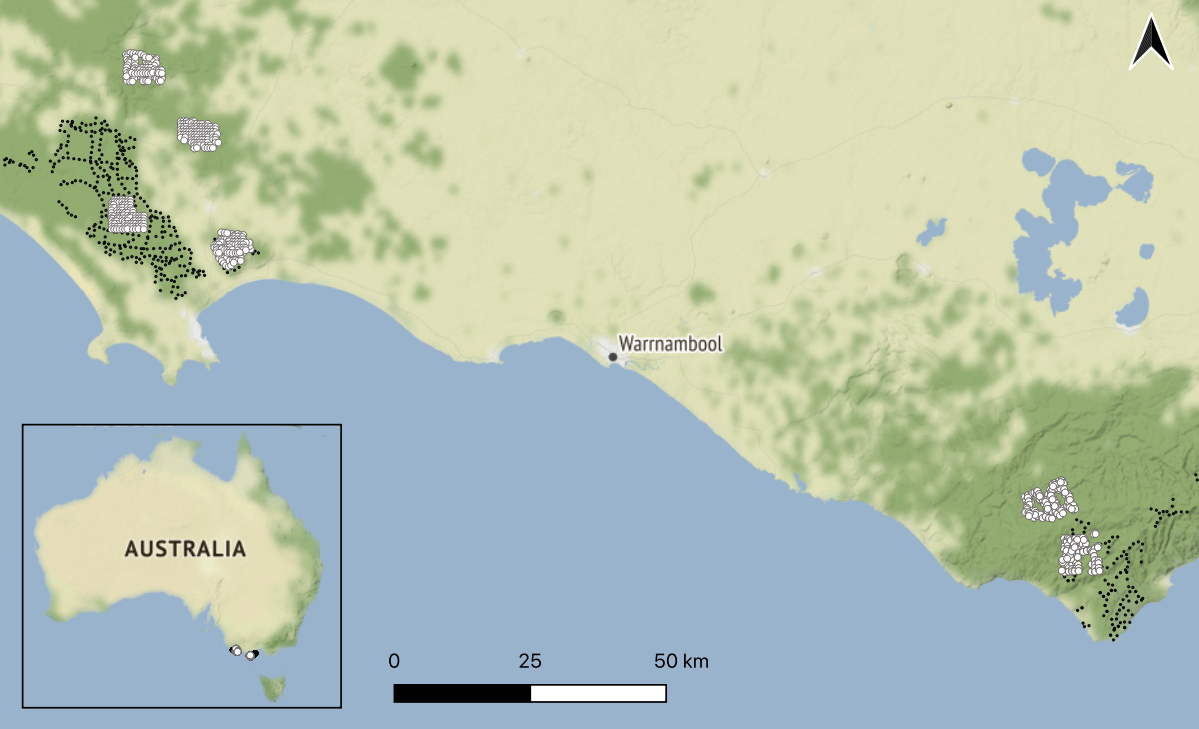
\includegraphics[width=1\linewidth]{figs/fig1} \caption{Locations of our six study landscapes in south-west Victoria, Australia. The grids of camera-traps are denoted by white dots, the locations of fox poison-bait stations are denoted by smaller black dots. The Glenelg region is to the west and Otway region to the east. Native vegetation is indicated by dark green, with hill shading. Map tiles by Stamen Design, under CC BY 3.0, map data by OpenStreetMap, under CC BY SA.}\label{fig:map}
\end{figure}

\newpage

\hypertarget{results}{%
\section{RESULTS}\label{results}}

\begin{longtable}[]{@{}cccccccc@{}}
\caption{\label{tab:sstab} Camera-trap surveys and feral cat spatial capture-recapture summary statistics.}\tabularnewline
\toprule
\begin{minipage}[b]{0.07\columnwidth}\centering
Land- scape\strut
\end{minipage} & \begin{minipage}[b]{0.08\columnwidth}\centering
Fox control?\strut
\end{minipage} & \begin{minipage}[b]{0.08\columnwidth}\centering
Camera- traps\strut
\end{minipage} & \begin{minipage}[b]{0.07\columnwidth}\centering
Trap nights\strut
\end{minipage} & \begin{minipage}[b]{0.09\columnwidth}\centering
Identified cats\strut
\end{minipage} & \begin{minipage}[b]{0.13\columnwidth}\centering
Identified detections\strut
\end{minipage} & \begin{minipage}[b]{0.14\columnwidth}\centering
Unidentified detections\strut
\end{minipage} & \begin{minipage}[b]{0.12\columnwidth}\centering
Unmarked detections\strut
\end{minipage}\tabularnewline
\midrule
\endfirsthead
\toprule
\begin{minipage}[b]{0.07\columnwidth}\centering
Land- scape\strut
\end{minipage} & \begin{minipage}[b]{0.08\columnwidth}\centering
Fox control?\strut
\end{minipage} & \begin{minipage}[b]{0.08\columnwidth}\centering
Camera- traps\strut
\end{minipage} & \begin{minipage}[b]{0.07\columnwidth}\centering
Trap nights\strut
\end{minipage} & \begin{minipage}[b]{0.09\columnwidth}\centering
Identified cats\strut
\end{minipage} & \begin{minipage}[b]{0.13\columnwidth}\centering
Identified detections\strut
\end{minipage} & \begin{minipage}[b]{0.14\columnwidth}\centering
Unidentified detections\strut
\end{minipage} & \begin{minipage}[b]{0.12\columnwidth}\centering
Unmarked detections\strut
\end{minipage}\tabularnewline
\midrule
\endhead
\begin{minipage}[t]{0.07\columnwidth}\centering
Annya\strut
\end{minipage} & \begin{minipage}[t]{0.08\columnwidth}\centering
no\strut
\end{minipage} & \begin{minipage}[t]{0.08\columnwidth}\centering
110\strut
\end{minipage} & \begin{minipage}[t]{0.07\columnwidth}\centering
8000\strut
\end{minipage} & \begin{minipage}[t]{0.09\columnwidth}\centering
9\strut
\end{minipage} & \begin{minipage}[t]{0.13\columnwidth}\centering
23\strut
\end{minipage} & \begin{minipage}[t]{0.14\columnwidth}\centering
3\strut
\end{minipage} & \begin{minipage}[t]{0.12\columnwidth}\centering
20\strut
\end{minipage}\tabularnewline
\begin{minipage}[t]{0.07\columnwidth}\centering
Cobbob\strut
\end{minipage} & \begin{minipage}[t]{0.08\columnwidth}\centering
yes\strut
\end{minipage} & \begin{minipage}[t]{0.08\columnwidth}\centering
110\strut
\end{minipage} & \begin{minipage}[t]{0.07\columnwidth}\centering
7752\strut
\end{minipage} & \begin{minipage}[t]{0.09\columnwidth}\centering
13\strut
\end{minipage} & \begin{minipage}[t]{0.13\columnwidth}\centering
35\strut
\end{minipage} & \begin{minipage}[t]{0.14\columnwidth}\centering
9\strut
\end{minipage} & \begin{minipage}[t]{0.12\columnwidth}\centering
37\strut
\end{minipage}\tabularnewline
\begin{minipage}[t]{0.07\columnwidth}\centering
Hotspur\strut
\end{minipage} & \begin{minipage}[t]{0.08\columnwidth}\centering
no\strut
\end{minipage} & \begin{minipage}[t]{0.08\columnwidth}\centering
99\strut
\end{minipage} & \begin{minipage}[t]{0.07\columnwidth}\centering
6085\strut
\end{minipage} & \begin{minipage}[t]{0.09\columnwidth}\centering
8\strut
\end{minipage} & \begin{minipage}[t]{0.13\columnwidth}\centering
22\strut
\end{minipage} & \begin{minipage}[t]{0.14\columnwidth}\centering
3\strut
\end{minipage} & \begin{minipage}[t]{0.12\columnwidth}\centering
13\strut
\end{minipage}\tabularnewline
\begin{minipage}[t]{0.07\columnwidth}\centering
Mt Clay\strut
\end{minipage} & \begin{minipage}[t]{0.08\columnwidth}\centering
yes\strut
\end{minipage} & \begin{minipage}[t]{0.08\columnwidth}\centering
106\strut
\end{minipage} & \begin{minipage}[t]{0.07\columnwidth}\centering
5451\strut
\end{minipage} & \begin{minipage}[t]{0.09\columnwidth}\centering
10\strut
\end{minipage} & \begin{minipage}[t]{0.13\columnwidth}\centering
33\strut
\end{minipage} & \begin{minipage}[t]{0.14\columnwidth}\centering
5\strut
\end{minipage} & \begin{minipage}[t]{0.12\columnwidth}\centering
0\strut
\end{minipage}\tabularnewline
\begin{minipage}[t]{0.07\columnwidth}\centering
South 2017\strut
\end{minipage} & \begin{minipage}[t]{0.08\columnwidth}\centering
no\strut
\end{minipage} & \begin{minipage}[t]{0.08\columnwidth}\centering
73\strut
\end{minipage} & \begin{minipage}[t]{0.07\columnwidth}\centering
3565\strut
\end{minipage} & \begin{minipage}[t]{0.09\columnwidth}\centering
20\strut
\end{minipage} & \begin{minipage}[t]{0.13\columnwidth}\centering
62\strut
\end{minipage} & \begin{minipage}[t]{0.14\columnwidth}\centering
8\strut
\end{minipage} & \begin{minipage}[t]{0.12\columnwidth}\centering
46\strut
\end{minipage}\tabularnewline
\begin{minipage}[t]{0.07\columnwidth}\centering
North 2017\strut
\end{minipage} & \begin{minipage}[t]{0.08\columnwidth}\centering
no\strut
\end{minipage} & \begin{minipage}[t]{0.08\columnwidth}\centering
67\strut
\end{minipage} & \begin{minipage}[t]{0.07\columnwidth}\centering
7099\strut
\end{minipage} & \begin{minipage}[t]{0.09\columnwidth}\centering
26\strut
\end{minipage} & \begin{minipage}[t]{0.13\columnwidth}\centering
60\strut
\end{minipage} & \begin{minipage}[t]{0.14\columnwidth}\centering
4\strut
\end{minipage} & \begin{minipage}[t]{0.12\columnwidth}\centering
48\strut
\end{minipage}\tabularnewline
\begin{minipage}[t]{0.07\columnwidth}\centering
South 2018\strut
\end{minipage} & \begin{minipage}[t]{0.08\columnwidth}\centering
yes\strut
\end{minipage} & \begin{minipage}[t]{0.08\columnwidth}\centering
85\strut
\end{minipage} & \begin{minipage}[t]{0.07\columnwidth}\centering
7838\strut
\end{minipage} & \begin{minipage}[t]{0.09\columnwidth}\centering
24\strut
\end{minipage} & \begin{minipage}[t]{0.13\columnwidth}\centering
75\strut
\end{minipage} & \begin{minipage}[t]{0.14\columnwidth}\centering
12\strut
\end{minipage} & \begin{minipage}[t]{0.12\columnwidth}\centering
62\strut
\end{minipage}\tabularnewline
\begin{minipage}[t]{0.07\columnwidth}\centering
North 2018\strut
\end{minipage} & \begin{minipage}[t]{0.08\columnwidth}\centering
no\strut
\end{minipage} & \begin{minipage}[t]{0.08\columnwidth}\centering
103\strut
\end{minipage} & \begin{minipage}[t]{0.07\columnwidth}\centering
4543\strut
\end{minipage} & \begin{minipage}[t]{0.09\columnwidth}\centering
30\strut
\end{minipage} & \begin{minipage}[t]{0.13\columnwidth}\centering
90\strut
\end{minipage} & \begin{minipage}[t]{0.14\columnwidth}\centering
17\strut
\end{minipage} & \begin{minipage}[t]{0.12\columnwidth}\centering
59\strut
\end{minipage}\tabularnewline
\begin{minipage}[t]{0.07\columnwidth}\centering
South 2019\strut
\end{minipage} & \begin{minipage}[t]{0.08\columnwidth}\centering
yes\strut
\end{minipage} & \begin{minipage}[t]{0.08\columnwidth}\centering
86\strut
\end{minipage} & \begin{minipage}[t]{0.07\columnwidth}\centering
6077\strut
\end{minipage} & \begin{minipage}[t]{0.09\columnwidth}\centering
25\strut
\end{minipage} & \begin{minipage}[t]{0.13\columnwidth}\centering
133\strut
\end{minipage} & \begin{minipage}[t]{0.14\columnwidth}\centering
22\strut
\end{minipage} & \begin{minipage}[t]{0.12\columnwidth}\centering
101\strut
\end{minipage}\tabularnewline
\begin{minipage}[t]{0.07\columnwidth}\centering
North 2019\strut
\end{minipage} & \begin{minipage}[t]{0.08\columnwidth}\centering
no\strut
\end{minipage} & \begin{minipage}[t]{0.08\columnwidth}\centering
99\strut
\end{minipage} & \begin{minipage}[t]{0.07\columnwidth}\centering
7150\strut
\end{minipage} & \begin{minipage}[t]{0.09\columnwidth}\centering
27\strut
\end{minipage} & \begin{minipage}[t]{0.13\columnwidth}\centering
90\strut
\end{minipage} & \begin{minipage}[t]{0.14\columnwidth}\centering
23\strut
\end{minipage} & \begin{minipage}[t]{0.12\columnwidth}\centering
58\strut
\end{minipage}\tabularnewline
\bottomrule
\end{longtable}

\emph{Note: There is a maximum of one detection per each 24-hour occasion.}

\begin{figure}
\includegraphics[width=1\linewidth]{figs/fig3_covs_600dpi} \caption{Fox probability of occupancy derived from generalised additive models within each impact (I) and associated non-impact (NI) landscape in the Glenelg (A) and Otways (B) regions. Estimates were used as predictor variables in the feral cat spatial mark-resight models.}\label{fig:foxplot}
\end{figure}

\newpage

\begin{longtable}[]{@{}ccccccc@{}}
\caption{\label{tab:aictab} Akaike's Information Criterion values adjusted for small sample size for top-5 ranked feral cat density models in each region (ordered in decreasing AICc scores).}\tabularnewline
\toprule
\begin{minipage}[b]{0.09\columnwidth}\centering
Region\strut
\end{minipage} & \begin{minipage}[b]{0.20\columnwidth}\centering
Density\strut
\end{minipage} & \begin{minipage}[b]{0.15\columnwidth}\centering
Detectability\strut
\end{minipage} & \begin{minipage}[b]{0.12\columnwidth}\centering
Parameters\strut
\end{minipage} & \begin{minipage}[b]{0.08\columnwidth}\centering
logLik\strut
\end{minipage} & \begin{minipage}[b]{0.07\columnwidth}\centering
dAICc\strut
\end{minipage} & \begin{minipage}[b]{0.08\columnwidth}\centering
AICcwt\strut
\end{minipage}\tabularnewline
\midrule
\endfirsthead
\toprule
\begin{minipage}[b]{0.09\columnwidth}\centering
Region\strut
\end{minipage} & \begin{minipage}[b]{0.20\columnwidth}\centering
Density\strut
\end{minipage} & \begin{minipage}[b]{0.15\columnwidth}\centering
Detectability\strut
\end{minipage} & \begin{minipage}[b]{0.12\columnwidth}\centering
Parameters\strut
\end{minipage} & \begin{minipage}[b]{0.08\columnwidth}\centering
logLik\strut
\end{minipage} & \begin{minipage}[b]{0.07\columnwidth}\centering
dAICc\strut
\end{minipage} & \begin{minipage}[b]{0.08\columnwidth}\centering
AICcwt\strut
\end{minipage}\tabularnewline
\midrule
\endhead
\begin{minipage}[t]{0.09\columnwidth}\centering
Glenelg\strut
\end{minipage} & \begin{minipage}[t]{0.20\columnwidth}\centering
fox\_occ\_avg\strut
\end{minipage} & \begin{minipage}[t]{0.15\columnwidth}\centering
1\strut
\end{minipage} & \begin{minipage}[t]{0.12\columnwidth}\centering
4\strut
\end{minipage} & \begin{minipage}[t]{0.08\columnwidth}\centering
-985.5\strut
\end{minipage} & \begin{minipage}[t]{0.07\columnwidth}\centering
0\strut
\end{minipage} & \begin{minipage}[t]{0.08\columnwidth}\centering
0.64\strut
\end{minipage}\tabularnewline
\begin{minipage}[t]{0.09\columnwidth}\centering
Glenelg\strut
\end{minipage} & \begin{minipage}[t]{0.20\columnwidth}\centering
fox\_occ\_avg\strut
\end{minipage} & \begin{minipage}[t]{0.15\columnwidth}\centering
fox\_occ\_avg\strut
\end{minipage} & \begin{minipage}[t]{0.12\columnwidth}\centering
6\strut
\end{minipage} & \begin{minipage}[t]{0.08\columnwidth}\centering
-984.4\strut
\end{minipage} & \begin{minipage}[t]{0.07\columnwidth}\centering
3.35\strut
\end{minipage} & \begin{minipage}[t]{0.08\columnwidth}\centering
0.12\strut
\end{minipage}\tabularnewline
\begin{minipage}[t]{0.09\columnwidth}\centering
Glenelg\strut
\end{minipage} & \begin{minipage}[t]{0.20\columnwidth}\centering
pair * foxbaited\_01\strut
\end{minipage} & \begin{minipage}[t]{0.15\columnwidth}\centering
1\strut
\end{minipage} & \begin{minipage}[t]{0.12\columnwidth}\centering
6\strut
\end{minipage} & \begin{minipage}[t]{0.08\columnwidth}\centering
-985\strut
\end{minipage} & \begin{minipage}[t]{0.07\columnwidth}\centering
4.4\strut
\end{minipage} & \begin{minipage}[t]{0.08\columnwidth}\centering
0.07\strut
\end{minipage}\tabularnewline
\begin{minipage}[t]{0.09\columnwidth}\centering
Glenelg\strut
\end{minipage} & \begin{minipage}[t]{0.20\columnwidth}\centering
pair + foxbaited\_01\strut
\end{minipage} & \begin{minipage}[t]{0.15\columnwidth}\centering
1\strut
\end{minipage} & \begin{minipage}[t]{0.12\columnwidth}\centering
5\strut
\end{minipage} & \begin{minipage}[t]{0.08\columnwidth}\centering
-986.5\strut
\end{minipage} & \begin{minipage}[t]{0.07\columnwidth}\centering
4.75\strut
\end{minipage} & \begin{minipage}[t]{0.08\columnwidth}\centering
0.06\strut
\end{minipage}\tabularnewline
\begin{minipage}[t]{0.09\columnwidth}\centering
Glenelg\strut
\end{minipage} & \begin{minipage}[t]{0.20\columnwidth}\centering
fox\_occ\strut
\end{minipage} & \begin{minipage}[t]{0.15\columnwidth}\centering
1\strut
\end{minipage} & \begin{minipage}[t]{0.12\columnwidth}\centering
4\strut
\end{minipage} & \begin{minipage}[t]{0.08\columnwidth}\centering
-988.3\strut
\end{minipage} & \begin{minipage}[t]{0.07\columnwidth}\centering
5.65\strut
\end{minipage} & \begin{minipage}[t]{0.08\columnwidth}\centering
0.04\strut
\end{minipage}\tabularnewline
\begin{minipage}[t]{0.09\columnwidth}\centering
Glenelg\strut
\end{minipage} & \begin{minipage}[t]{0.20\columnwidth}\centering
foxbaited\_01\strut
\end{minipage} & \begin{minipage}[t]{0.15\columnwidth}\centering
1\strut
\end{minipage} & \begin{minipage}[t]{0.12\columnwidth}\centering
4\strut
\end{minipage} & \begin{minipage}[t]{0.08\columnwidth}\centering
-988.9\strut
\end{minipage} & \begin{minipage}[t]{0.07\columnwidth}\centering
6.91\strut
\end{minipage} & \begin{minipage}[t]{0.08\columnwidth}\centering
0.02\strut
\end{minipage}\tabularnewline
\begin{minipage}[t]{0.09\columnwidth}\centering
Otways\strut
\end{minipage} & \begin{minipage}[t]{0.20\columnwidth}\centering
fox\_occ\strut
\end{minipage} & \begin{minipage}[t]{0.15\columnwidth}\centering
fox\_occ\strut
\end{minipage} & \begin{minipage}[t]{0.12\columnwidth}\centering
6\strut
\end{minipage} & \begin{minipage}[t]{0.08\columnwidth}\centering
-3543\strut
\end{minipage} & \begin{minipage}[t]{0.07\columnwidth}\centering
0\strut
\end{minipage} & \begin{minipage}[t]{0.08\columnwidth}\centering
0.37\strut
\end{minipage}\tabularnewline
\begin{minipage}[t]{0.09\columnwidth}\centering
Otways\strut
\end{minipage} & \begin{minipage}[t]{0.20\columnwidth}\centering
1\strut
\end{minipage} & \begin{minipage}[t]{0.15\columnwidth}\centering
fox\_occ\strut
\end{minipage} & \begin{minipage}[t]{0.12\columnwidth}\centering
5\strut
\end{minipage} & \begin{minipage}[t]{0.08\columnwidth}\centering
-3545\strut
\end{minipage} & \begin{minipage}[t]{0.07\columnwidth}\centering
1.58\strut
\end{minipage} & \begin{minipage}[t]{0.08\columnwidth}\centering
0.17\strut
\end{minipage}\tabularnewline
\begin{minipage}[t]{0.09\columnwidth}\centering
Otways\strut
\end{minipage} & \begin{minipage}[t]{0.20\columnwidth}\centering
1\strut
\end{minipage} & \begin{minipage}[t]{0.15\columnwidth}\centering
fox\_occ\_avg\strut
\end{minipage} & \begin{minipage}[t]{0.12\columnwidth}\centering
5\strut
\end{minipage} & \begin{minipage}[t]{0.08\columnwidth}\centering
-3545\strut
\end{minipage} & \begin{minipage}[t]{0.07\columnwidth}\centering
2.27\strut
\end{minipage} & \begin{minipage}[t]{0.08\columnwidth}\centering
0.12\strut
\end{minipage}\tabularnewline
\begin{minipage}[t]{0.09\columnwidth}\centering
Otways\strut
\end{minipage} & \begin{minipage}[t]{0.20\columnwidth}\centering
fox\_occ\_avg\strut
\end{minipage} & \begin{minipage}[t]{0.15\columnwidth}\centering
fox\_occ\_avg\strut
\end{minipage} & \begin{minipage}[t]{0.12\columnwidth}\centering
6\strut
\end{minipage} & \begin{minipage}[t]{0.08\columnwidth}\centering
-3544\strut
\end{minipage} & \begin{minipage}[t]{0.07\columnwidth}\centering
2.44\strut
\end{minipage} & \begin{minipage}[t]{0.08\columnwidth}\centering
0.11\strut
\end{minipage}\tabularnewline
\begin{minipage}[t]{0.09\columnwidth}\centering
Otways\strut
\end{minipage} & \begin{minipage}[t]{0.20\columnwidth}\centering
1\strut
\end{minipage} & \begin{minipage}[t]{0.15\columnwidth}\centering
foxbaited\_01\strut
\end{minipage} & \begin{minipage}[t]{0.12\columnwidth}\centering
5\strut
\end{minipage} & \begin{minipage}[t]{0.08\columnwidth}\centering
-3546\strut
\end{minipage} & \begin{minipage}[t]{0.07\columnwidth}\centering
3.64\strut
\end{minipage} & \begin{minipage}[t]{0.08\columnwidth}\centering
0.06\strut
\end{minipage}\tabularnewline
\begin{minipage}[t]{0.09\columnwidth}\centering
Otways\strut
\end{minipage} & \begin{minipage}[t]{0.20\columnwidth}\centering
grid + before\_after\strut
\end{minipage} & \begin{minipage}[t]{0.15\columnwidth}\centering
foxbaited\_01\strut
\end{minipage} & \begin{minipage}[t]{0.12\columnwidth}\centering
7\strut
\end{minipage} & \begin{minipage}[t]{0.08\columnwidth}\centering
-3544\strut
\end{minipage} & \begin{minipage}[t]{0.07\columnwidth}\centering
3.8\strut
\end{minipage} & \begin{minipage}[t]{0.08\columnwidth}\centering
0.06\strut
\end{minipage}\tabularnewline
\begin{minipage}[t]{0.09\columnwidth}\centering
Otways\strut
\end{minipage} & \begin{minipage}[t]{0.20\columnwidth}\centering
foxbaited\_01\strut
\end{minipage} & \begin{minipage}[t]{0.15\columnwidth}\centering
foxbaited\_01\strut
\end{minipage} & \begin{minipage}[t]{0.12\columnwidth}\centering
6\strut
\end{minipage} & \begin{minipage}[t]{0.08\columnwidth}\centering
-3545\strut
\end{minipage} & \begin{minipage}[t]{0.07\columnwidth}\centering
3.89\strut
\end{minipage} & \begin{minipage}[t]{0.08\columnwidth}\centering
0.05\strut
\end{minipage}\tabularnewline
\begin{minipage}[t]{0.09\columnwidth}\centering
Otways\strut
\end{minipage} & \begin{minipage}[t]{0.20\columnwidth}\centering
grid * before\_after\strut
\end{minipage} & \begin{minipage}[t]{0.15\columnwidth}\centering
foxbaited\_01\strut
\end{minipage} & \begin{minipage}[t]{0.12\columnwidth}\centering
8\strut
\end{minipage} & \begin{minipage}[t]{0.08\columnwidth}\centering
-3543\strut
\end{minipage} & \begin{minipage}[t]{0.07\columnwidth}\centering
5.76\strut
\end{minipage} & \begin{minipage}[t]{0.08\columnwidth}\centering
0.02\strut
\end{minipage}\tabularnewline
\begin{minipage}[t]{0.09\columnwidth}\centering
Otways\strut
\end{minipage} & \begin{minipage}[t]{0.20\columnwidth}\centering
grid + year\strut
\end{minipage} & \begin{minipage}[t]{0.15\columnwidth}\centering
foxbaited\_01\strut
\end{minipage} & \begin{minipage}[t]{0.12\columnwidth}\centering
8\strut
\end{minipage} & \begin{minipage}[t]{0.08\columnwidth}\centering
-3543\strut
\end{minipage} & \begin{minipage}[t]{0.07\columnwidth}\centering
5.89\strut
\end{minipage} & \begin{minipage}[t]{0.08\columnwidth}\centering
0.02\strut
\end{minipage}\tabularnewline
\begin{minipage}[t]{0.09\columnwidth}\centering
Otways\strut
\end{minipage} & \begin{minipage}[t]{0.20\columnwidth}\centering
fox\_occ\strut
\end{minipage} & \begin{minipage}[t]{0.15\columnwidth}\centering
1\strut
\end{minipage} & \begin{minipage}[t]{0.12\columnwidth}\centering
4\strut
\end{minipage} & \begin{minipage}[t]{0.08\columnwidth}\centering
-3548\strut
\end{minipage} & \begin{minipage}[t]{0.07\columnwidth}\centering
6.65\strut
\end{minipage} & \begin{minipage}[t]{0.08\columnwidth}\centering
0.01\strut
\end{minipage}\tabularnewline
\bottomrule
\end{longtable}

\newpage

\begin{figure}
\includegraphics[width=1\linewidth]{figs/fig3_glenelg_600dpi} \caption{Best-ranked experimental (A) and correlative (B) models of feral cat density in the Glenelg region, Australia. There was statistical evidence (i.e., 95\% confidence intervals of the parameter estimates did not overlap zero) that feral cat density was higher in the landscape with fox-baiting (impact) than the associated landscape without fox-baiting (non-impact) for the first replicate, but not for the second replicate (A). The best-ranked model predicted that feral cat density declined with the probability of fox occupancy at the landscape level (B). Error bars and the shaded region indicate 95\% confidence intervals.}\label{fig:gplots}
\end{figure}

\begin{figure}
\includegraphics[width=1\linewidth]{figs/fig4_otway_600dpi} \caption{Best-ranked model of feral cat density in the Otway region, Australia. The best-ranked model predicted that feral cat density declined with the probability of fox occupancy (B). This model also predicted that the probability of detecting a feral cat in its activity centre per 24-hour occasion (g0) increased with the probability of fox occupancy (B), while sigma (which is related to home range size) increased (C). Shaded regions indicate 95\% confidence intervals.}\label{fig:oplots}
\end{figure}

\newpage

\hypertarget{discussion}{%
\section{DISCUSSION}\label{discussion}}

\newpage

\hypertarget{conclusions}{%
\section{CONCLUSIONS}\label{conclusions}}

\newpage

\hypertarget{acknowledgements}{%
\section{ACKNOWLEDGEMENTS}\label{acknowledgements}}

We acknowledge and pay respect to the Gadubanud and Gunditjmara people on whose traditional lands this study took place. Surveys were conducted under University of Melbourne Animal Ethics Committee approval 1714119 and Victorian Government Department of Environment, Land Water and Planning Research Permit 10008273. This experiment was a collaborative effort between the Glenelg Ark (Department of Environment, Land Water and Planning) and Otway Ark (Parks Victoria) working groups.
We are extremely grateful to our field assistants: Shauni Omond, Shayne Neal, Asitha Samarawickrama, Shelley Thompson, Erin Harris, Hannah Killian, Lani Watson, Mark Dorman, Jack Davis, Carl Roffey, Bruce Edley, Larissa Oliveira Gonçalves, Ben Lake, Chantelle Geissler, Aviya Naccarella, Emily Gronow, Harley England, David Pitts, Annie Hobby, Louise Falls, Thomas McKinnon, Jimmy Downie, Marney Hradsky, Stephanie Samson, Robin Sinclair, Asmaa Alhusainan, Kelly Forrester, Tammana Wadawani, Emily McColl-Gausden, Emily Gregg, Hannah Edwards, Adam Beck, Vishnu Memnon, Sandy Lu, Pia Lentini, Nick Golding, Emily McColl-Gausden, Nina Page, Maggie Campbell-Jones, Kyle Quinn and Jack Dickson. This manuscript was improved by comments from William Geary. Our study was generously supported by the Conservation Ecology Centre, the Victorian Government Department of Environment, Land Water and Planning, Arthur Rylah Institute for Environmental Research, Parks Victoria and the Australian Government's National Environmental Science Program through the Threatened Species Recovery Hub, and ARC Linkage Project LP170101134. MR also receives support from an Australian Government Research Training Program Scholarship.

\hypertarget{authors-contributions}{%
\section{AUTHORS' CONTRIBUTIONS}\label{authors-contributions}}

M.W.R, B.H, J.H.P, B.A.W and A.R conceived the ideas and designed methodology; M.W.R, J.H.P, M.LP, E.K.B and B.H collected the data; M.W.R analysed the data; M.W.R led the writing of the manuscript. All authors contributed critically to the drafts and gave final approval for publication.

\hypertarget{open-research}{%
\section{OPEN RESEARCH}\label{open-research}}

Raw data and code are on Github link xx.\\
Data will be deposited on the Dryad Digital Repository after acceptance.

\newpage

\hypertarget{references}{%
\section*{REFERENCES}\label{references}}
\addcontentsline{toc}{section}{REFERENCES}

\hypertarget{refs}{}
\leavevmode\hypertarget{ref-alston2019}{}%
Alston, J., Maitland, B., Brito, B., Esmaeili, S., Ford, A., Hays, B., Jesmer, B., Molina, F., \& Goheen, J. (2019). Reciprocity in restoration ecology: When might large carnivore reintroduction restore ecosystems? \emph{Biological Conservation}, \emph{234}, 82--89.

\leavevmode\hypertarget{ref-ballari2016}{}%
Ballari, S. A., Kuebbing, S. E., \& Nuñez, M. A. (2016). Potential problems of removing one invasive species at a time: A meta-analysis of the interactions between invasive vertebrates and unexpected effects of removal programs. \emph{PeerJ}, \emph{4}, e2029.

\leavevmode\hypertarget{ref-bode2015}{}%
Bode, M., Baker, C. M., \& Plein, M. (2015). Eradicating down the food chain: Optimal multispecies eradication schedules for a commonly encountered invaded island ecosystem. \emph{Journal of Applied Ecology}, \emph{52}(3), 571--579.

\leavevmode\hypertarget{ref-borchers2008}{}%
Borchers, D. L., \& Efford, M. G. (2008). Spatially explicit maximum likelihood methods for capture--recapture studies. \emph{Biometrics}, \emph{64}(2), 377--385.

\leavevmode\hypertarget{ref-broadley2019}{}%
Broadley, K., Burton, A. C., Avgar, T., \& Boutin, S. (2019). Density-dependent space use affects interpretation of camera trap detection rates. \emph{Ecology and Evolution}, \emph{9}(24), 14031--14041.

\leavevmode\hypertarget{ref-BOM2021}{}%
\emph{Bureau of meteorology}. (2021). Climate Data Online URL; (accessed May 2021). \url{http://www.bom.gov.au/climate/data/}

\leavevmode\hypertarget{ref-burnham2004}{}%
Burnham, K. P., \& Anderson, D. R. (2004). Multimodel inference: Understanding aic and bic in model selection. \emph{Sociological Methods \& Research}, \emph{33}(2), 261--304.

\leavevmode\hypertarget{ref-catling1988}{}%
Catling, P. (1988). Similarities and contrasts in the diets of foxes, vulpes vulpes, and cats, felis catus, relative to fluctuating prey populations and drought. \emph{Wildlife Research}, \emph{15}(3), 307--317.

\leavevmode\hypertarget{ref-christie2019}{}%
Christie, A. P., Amano, T., Martin, P. A., Shackelford, G. E., Simmons, B. I., \& Sutherland, W. J. (2019). Simple study designs in ecology produce inaccurate estimates of biodiversity responses. \emph{Journal of Applied Ecology}, \emph{56}(12), 2742--2754.

\leavevmode\hypertarget{ref-claridge2010}{}%
Claridge, A. W., Cunningham, R. B., Catling, P. C., \& Reid, A. M. (2010). Trends in the activity levels of forest-dwelling vertebrate fauna against a background of intensive baiting for foxes. \emph{Forest Ecology and Management}, \emph{260}(5), 822--832.

\leavevmode\hypertarget{ref-courchamp1999}{}%
Courchamp, F., Langlais, M., \& Sugihara, G. (1999). Cats protecting birds: Modelling the mesopredator release effect. \emph{Journal of Animal Ecology}, \emph{68}(2), 282--292.

\leavevmode\hypertarget{ref-crooks1999}{}%
Crooks, K. R., \& Soulé, M. E. (1999). Mesopredator release and avifaunal extinctions in a fragmented system. \emph{Nature}, \emph{400}(6744), 563--566.

\leavevmode\hypertarget{ref-davey2006}{}%
Davey, C., Sinclair, A., Pech, R. P., Arthur, A. D., Krebs, C. J., Newsome, A., Hik, D., Molsher, R., \& Allcock, K. (2006). Do exotic vertebrates structure the biota of australia? An experimental test in new south wales. \emph{Ecosystems}, \emph{9}(6), 992--1008.

\leavevmode\hypertarget{ref-delwp2020}{}%
DELWP. (2020). \emph{Bioregions and evc benchmarks}. Victorian Government Department of Environment, Land, Water; Planning, Melbourne. Accessed June 2021). \url{https://www.environment.vic.gov.au/biodiversity/bioregions-and-evc-benchmarks}

\leavevmode\hypertarget{ref-doherty2017}{}%
Doherty, T. S., \& Ritchie, E. G. (2017). Stop jumping the gun: A call for evidence-based invasive predator management. \emph{Conservation Letters}, \emph{10}(1), 15--22.

\leavevmode\hypertarget{ref-efford2021secr}{}%
Efford, M. G. (2021). \emph{Secr: Spatially explicit capture-recapture models. R package version 4.4.4}. (accessed June 2021). \url{http://CRAN.R-project.org/package=secr}

\leavevmode\hypertarget{ref-efford2012}{}%
Efford, M. G., \& Dawson, D. K. (2012). Occupancy in continuous habitat. \emph{Ecosphere}, \emph{3}(4), 1--15.

\leavevmode\hypertarget{ref-finke2004}{}%
Finke, D. L., \& Denno, R. F. (2004). Predator diversity dampens trophic cascades. \emph{Nature}, \emph{429}(6990), 407--410.

\leavevmode\hypertarget{ref-fisher2015}{}%
Fisher, P., Algar, D., Murphy, E., Johnston, M., \& Eason, C. (2015). How does cat behaviour influence the development and implementation of monitoring techniques and lethal control methods for feral cats? \emph{Applied Animal Behaviour Science}, \emph{173}, 88--96.

\leavevmode\hypertarget{ref-forsyth2019}{}%
Forsyth, D. M., Ramsey, D. S., \& Woodford, L. P. (2019). Estimating abundances, densities, and interspecific associations in a carnivore community. \emph{The Journal of Wildlife Management}, \emph{83}(5), 1090--1102.

\leavevmode\hypertarget{ref-glen2011}{}%
Glen, A., Pennay, M., Dickman, C., Wintle, B., \& Firestone, K. (2011). Diets of sympatric native and introduced carnivores in the barrington tops, eastern australia. \emph{Austral Ecology}, \emph{36}(3), 290--296.

\leavevmode\hypertarget{ref-glen2005}{}%
Glen, A. S., \& Dickman, C. R. (2005). Complex interactions among mammalian carnivores in australia, and their implications for wildlife management. \emph{Biological Reviews}, \emph{80}(3), 387--401.

\leavevmode\hypertarget{ref-hastings2001}{}%
Hastings, A. (2001). Transient dynamics and persistence of ecological systems. \emph{Ecology Letters}, \emph{4}(3), 215--220.

\leavevmode\hypertarget{ref-hayward2015}{}%
Hayward, M. W., Boitani, L., Burrows, N. D., Funston, P. J., Karanth, K. U., MacKenzie, D. I., Pollock, K. H., \& Yarnell, R. W. (2015). Ecologists need robust survey designs, sampling and analytical methods. \emph{Journal of Applied Ecology}, \emph{52}(2), 286--290.

\leavevmode\hypertarget{ref-hradsky2017human}{}%
Hradsky, B. A., Robley, A., Alexander, R., Ritchie, E. G., York, A., \& Di Stefano, J. (2017). Human-modified habitats facilitate forest-dwelling populations of an invasive predator, vulpes vulpes. \emph{Scientific Reports}, \emph{7}(1), 1--12.

\leavevmode\hypertarget{ref-hunter2018}{}%
Hunter, D. O., Lagisz, M., Leo, V., Nakagawa, S., \& Letnic, M. (2018). Not all predators are equal: A continent-scale analysis of the effects of predator control on australian mammals. \emph{Mammal Review}, \emph{48}(2), 108--122.

\leavevmode\hypertarget{ref-jackson2015}{}%
Jackson, M. C. (2015). Interactions among multiple invasive animals. \emph{Ecology}, \emph{96}(8), 2035--2041.

\leavevmode\hypertarget{ref-kuebbing2015}{}%
Kuebbing, S. E., \& Nuñez, M. A. (2015). Negative, neutral, and positive interactions among nonnative plants: Patterns, processes, and management implications. \emph{Global Change Biology}, \emph{21}(2), 926--934.

\leavevmode\hypertarget{ref-lazenby2015}{}%
Lazenby, B. T., Mooney, N. J., \& Dickman, C. R. (2015). Effects of low-level culling of feral cats in open populations: A case study from the forests of southern tasmania. \emph{Wildlife Research}, \emph{41}(5), 407--420.

\leavevmode\hypertarget{ref-legge2020}{}%
Legge, S., Taggart, P. L., Dickman, C. R., Read, J. L., \& Woinarski, J. C. (2020). \emph{Wildlife Research}, \emph{47}(8), 731--746.

\leavevmode\hypertarget{ref-marlow2015}{}%
Marlow, N. J., Thomas, N. D., Williams, A. A., Macmahon, B., Lawson, J., Hitchen, Y., Angus, J., \& Berry, O. (2015). Cats (felis catus) are more abundant and are the dominant predator of woylies (bettongia penicillata) after sustained fox (vulpes vulpes) control. \emph{Australian Journal of Zoology}, \emph{63}(1), 18--27.

\leavevmode\hypertarget{ref-mcleod2014}{}%
McLeod, S. R., \& Saunders, G. (2014). Fertility control is much less effective than lethal baiting for controlling foxes. \emph{Ecological Modelling}, \emph{273}, 1--10.

\leavevmode\hypertarget{ref-medina2011}{}%
Medina, F. M., Bonnaud, E., Vidal, E., Tershy, B. R., Zavaleta, E. S., Josh Donlan, C., Keitt, B. S., Le Corre, M., Horwath, S. V., \& Nogales, M. (2011). A global review of the impacts of invasive cats on island endangered vertebrates. \emph{Global Change Biology}, \emph{17}(11), 3503--3510.

\leavevmode\hypertarget{ref-miller2014}{}%
Miller, D. L., \& Wood, S. N. (2014). Finite area smoothing with generalized distance splines. \emph{Environmental and Ecological Statistics}, \emph{21}(4), 715--731.

\leavevmode\hypertarget{ref-molsher2017}{}%
Molsher, R., Newsome, A. E., Newsome, T. M., \& Dickman, C. R. (2017). Mesopredator management: Effects of red fox control on the abundance, diet and use of space by feral cats. \emph{PLoS One}, \emph{12}(1), e0168460.

\leavevmode\hypertarget{ref-moseby2019}{}%
Moseby, K. E., Letnic, M., Blumstein, D. T., \& West, R. (2019). Understanding predator densities for successful co-existence of alien predators and threatened prey. \emph{Austral Ecology}, \emph{44}(3), 409--419.

\leavevmode\hypertarget{ref-moseby2020effectiveness}{}%
Moseby, K., McGregor, H., \& Read, J. (2020). Effectiveness of the felixer grooming trap for the control of feral cats: A field trial in arid south australia. \emph{Wildlife Research}, \emph{47}(8), 599--609.

\leavevmode\hypertarget{ref-niedballa2016}{}%
Niedballa, J., Sollmann, R., Courtiol, A., \& Wilting, A. (2016). CamtrapR: An r package for efficient camera trap data management. \emph{Methods in Ecology and Evolution}, \emph{7}(12), 1457--1462.

\leavevmode\hypertarget{ref-rayner2007}{}%
Rayner, M. J., Hauber, M. E., Imber, M. J., Stamp, R. K., \& Clout, M. N. (2007). Spatial heterogeneity of mesopredator release within an oceanic island system. \emph{Proceedings of the National Academy of Sciences}, \emph{104}(52), 20862--20865.

\leavevmode\hypertarget{ref-reddiex2007}{}%
Reddiex, B., Forsyth, D. M., McDonald-Madden, E., Einoder, L. D., Griffioen, P. A., Chick, R. R., \& Robley, A. J. (2007). Control of pest mammals for biodiversity protection in australia. I. Patterns of control and monitoring. \emph{Wildlife Research}, \emph{33}(8), 691--709.

\leavevmode\hypertarget{ref-rees2019}{}%
Rees, M., Pascoe, J., Wintle, B., Le Pla, M., Birnbaum, E., \& Hradsky, B. (2019). Unexpectedly high densities of feral cats in a rugged temperate forest. \emph{Biological Conservation}, \emph{239}, 108287.

\leavevmode\hypertarget{ref-riley1999}{}%
Riley, S. J., DeGloria, S. D., \& Elliot, R. (1999). Index that quantifies topographic heterogeneity. \emph{Intermountain Journal of Sciences}, \emph{5}(1-4), 23--27.

\leavevmode\hypertarget{ref-risbey2000}{}%
Risbey, D. A., Calver, M. C., Short, J., Bradley, J. S., \& Wright, I. W. (2000). The impact of cats and foxes on the small vertebrate fauna of heirisson prong, western australia. II. A field experiment. \emph{Wildlife Research}, \emph{27}(3), 223--235.

\leavevmode\hypertarget{ref-robley2014}{}%
Robley, A., Gormley, A. M., Forsyth, D. M., \& Triggs, B. (2014). Long-term and large-scale control of the introduced red fox increases native mammal occupancy in australian forests. \emph{Biological Conservation}, \emph{180}, 262--269.

\leavevmode\hypertarget{ref-rogan2019}{}%
Rogan, M. S., Balme, G. A., Distiller, G., Pitman, R. T., Broadfield, J., Mann, G. K., Whittington-Jones, G. M., Thomas, L. H., \& O'Riain, M. J. (2019). The influence of movement on the occupancy--density relationship at small spatial scales. \emph{Ecosphere}, \emph{10}(8), e02807.

\leavevmode\hypertarget{ref-ruscoe2011}{}%
Ruscoe, W. A., Ramsey, D. S., Pech, R. P., Sweetapple, P. J., Yockney, I., Barron, M. C., Perry, M., Nugent, G., Carran, R., Warne, R., \& others. (2011). Unexpected consequences of control: Competitive vs. Predator release in a four-species assemblage of invasive mammals. \emph{Ecology Letters}, \emph{14}(10), 1035--1042.

\leavevmode\hypertarget{ref-short1999}{}%
Short, J., Calver, M. C., \& Risbey, D. A. (1999). The impact of cats and foxes on the small vertebrate fauna of heirisson prong, western australia. I. Exploring potential impact using diet analysis. \emph{Wildlife Research}, \emph{26}(5), 621--630.

\leavevmode\hypertarget{ref-smith2020}{}%
Smith, J. A., Suraci, J. P., Hunter, J. S., Gaynor, K. M., Keller, C. B., Palmer, M. S., Atkins, J. L., Castañeda, I., Cherry, M. J., Garvey, P. M., \& others. (2020). Zooming in on mechanistic predator--prey ecology: Integrating camera traps with experimental methods to reveal the drivers of ecological interactions. \emph{Journal of Animal Ecology}, \emph{89}(9), 1997--2012.

\leavevmode\hypertarget{ref-soule1988}{}%
Soulé, M. E., Bolger, D. T., Alberts, A. C., Wrights, J., Sorice, M., \& Hill, S. (1988). Reconstructed dynamics of rapid extinctions of chaparral-requiring birds in urban habitat islands. \emph{Conservation Biology}, \emph{2}(1), 75--92.

\leavevmode\hypertarget{ref-stephens2015}{}%
Stephens, P. A., Pettorelli, N., Barlow, J., Whittingham, M. J., \& Cadotte, M. W. (2015). \emph{Management by proxy? The use of indices in applied ecology}. Wiley Online Library.

\leavevmode\hypertarget{ref-stobo2020management}{}%
Stobo-Wilson, A. M., Brandle, R., Johnson, C. N., \& Jones, M. E. (2020). Management of invasive mesopredators in the flinders ranges, south australia: Effectiveness and implications. \emph{Wildlife Research}, \emph{47}(8), 720--730.

\leavevmode\hypertarget{ref-towerton2011}{}%
Towerton, A. L., Penman, T. D., Kavanagh, R. P., \& Dickman, C. R. (2011). Detecting pest and prey responses to fox control across the landscape using remote cameras. \emph{Wildlife Research}, \emph{38}(3), 208--220.

\leavevmode\hypertarget{ref-wood2011}{}%
Wood, S. N. (2011). Fast stable restricted maximum likelihood and marginal likelihood estimation of semiparametric generalized linear models. \emph{Journal of the Royal Statistical Society: Series B (Statistical Methodology)}, \emph{73}(1), 3--36.

\leavevmode\hypertarget{ref-wood2017}{}%
Wood, S. N. (2017). \emph{Generalized additive models: An introduction with r}. CRC press.

\leavevmode\hypertarget{ref-zavaleta2001}{}%
Zavaleta, E. S., Hobbs, R. J., \& Mooney, H. A. (2001). Viewing invasive species removal in a whole-ecosystem context. \emph{Trends in Ecology \& Evolution}, \emph{16}(8), 454--459.


\end{document}


